\section{Generalization and acceptability}

The BNC2014 analysis asks whether the production profile travels across corpus
design, variety, period, and annotation regime. The transport model is trained
on the spoken \texttt{languageR} rows restricted to the six BNC2014 verbs. It's
then evaluated on harmonized BNC2014 rows, with complete-case filtering stated
as part of the evidential scope.

Three estimands are kept apart. The \texttt{languageR} models estimate
conditional production choice among attested noun phrase and prepositional
phrase dative tokens. The BNC2014 transport result estimates out-of-domain
predictive performance over complete-case rows in the six shared
high-frequency verbs after harmonization. DAIS estimates controlled
double-object preference for constructed alternatives. These numbers can
therefore be read together only as different evidence channels, not as repeated
measurements of one quantity.

Cross-variety probabilistic grammar of the dative isn't new ground.
\textcite{BresnanFord2010} compared American and Australian English and found
that speakers' probabilistic choice knowledge is largely shared across
varieties, but varies enough to surface in naturalness ratings and
lexical-decision latencies. \textcite{RothlisbergerGrafmillerSzmrecsanyi2017}
extended the comparison across nine post-colonial Englishes and found broad
stability with local traces of indigenization. So the bare finding that dative
conditioning largely travels wouldn't, on its own, be new.

Two things here are different. First, it's a strict out-of-domain test: one
model is fit on one corpus and scored on another against held-out log loss, area
under the curve, and scrambled-label nulls, rather than fit separately within
each variety. Second, the transport result feeds a distinction the variationist
work doesn't draw, between production probability and grammatical possibility,
developed in the next section. The contribution is that framing and the test, not
the stability itself.

The comparison is therefore an out-of-domain transport test. The first
transport model holds modality close by training only on spoken
\texttt{languageR} rows, but the corpus shift is still large: American
telephone conversation from 1990--1991 to spontaneous British conversation from
2012--2014, under a different annotation scheme and a six-verb target set.
That target set is already a scope restriction. In \texttt{languageR}, those six
verbs account for 2,201 of 3,263 rows, and for 1,564 of 2,360 spoken rows. They
are the high-frequency core, not a random sample of the alternation.

Harmonization is lossy. The outcome maps cleanly: \texttt{VNN} becomes NP and
\texttt{VNPP} becomes PP. Verb also maps cleanly after restricting the
\texttt{languageR} data to the six shared verbs. Length needs more care. The
released BNC2014 length fields are character counts: the data dictionary defines
\texttt{RecLen} and \texttt{ThemeLen} as the number of characters in the
recipient and theme \citep{JensetMcGillivray2019Dative}. Those aren't comparable
to \texttt{languageR}'s token-like lengths, so the released fields can't enter
the transport model directly. The script instead derives word counts from the
recipient and theme strings. Two costs follow: the whitespace tokenization isn't
guaranteed to match the convention behind \texttt{languageR}'s counts, and the
few rows with empty phrase strings drop out, since a character count can't be
turned back into a word count.

Several predictors are available only as proxies. BNC2014 has recipient and
theme animacy, theme definiteness, and recipient/theme pronominality, but some
fields have missing values and different annotation paths. Recipient
definiteness is not released as a field, so it enters only as a labelled regex
proxy in a sensitivity check. Discourse accessibility is unavailable and is
dropped from transport.

The core transport model therefore scores the 1,621 BNC2014 rows complete for
the harmonized predictors, not all 1,839 released dative rows. The missing rows
are not neutral: noun phrase recipients make up 0.819 of the complete rows but
only 0.670 of the 218 incomplete rows. The headline comparison is consequently
a complete-case estimate over the shared high-frequency core.

A BNC2014 metadata audit makes the domain label concrete. In the released
dative rows, Level 1 dialect is \enquote{uk} for 1,720 of 1,839 rows and Level 2
dialect is \enquote{english} for 1,689. Gender is female-coded for 1,138 rows
and male-coded for 699, and the largest age band is 19--29 with 736 rows.
Interaction type is also skewed: close-family, partner, and very-close-friend
conversations contribute 1,171 rows, while friends and wider-family
conversations contribute another 538. The complete-case subset has the same
shape. A single BNC2014 transport score should therefore be read as a
corpus-domain diagnostic, not as a clean estimate for British spoken English in
general.

\begin{table}[htbp]
\centering
\small
\begin{tabular}{>{\raggedright\arraybackslash}p{0.48\linewidth}>{\raggedright\arraybackslash}p{0.22\linewidth}rr}
\toprule
Model & Test data & Log loss & AUC \\
\midrule
\texttt{languageR} marginal & BNC2014 complete & 0.473 & 0.500 \\
\texttt{languageR} core transport & BNC2014 complete & 0.308 & 0.906 \\
\texttt{languageR} core transport & Scrambled BNC2014 complete & 0.885 & 0.515 \\
BNC2014 marginal holdout & BNC2014 complete & 0.481 & 0.500 \\
BNC2014 native core holdout & BNC2014 complete & 0.202 & 0.960 \\
BNC2014 native scrambled train & BNC2014 complete & 0.495 & 0.440 \\
\bottomrule
\end{tabular}
\caption{First BNC2014 complete-case transport and native holdout comparisons.}
\label{tab:bnc-transport}
\end{table}

The transported core model beats the marginal baseline by a wide margin. Its
test log loss is 0.308, compared with 0.473 for the \texttt{languageR} marginal
baseline, and its AUC is 0.906. A percentile bootstrap over the BNC2014
complete-case test rows (2,000 resamples) puts the log loss in [0.277, 0.337]
and the AUC in [0.890, 0.922], so the result isn't an artefact of one lucky
split. When the BNC2014 outcome is scrambled, the same predictions collapse to
0.885 log loss and 0.515 AUC.

Simple all-row imputation checks make the complete-case scope visible. With
missing lengths set to their BNC2014 medians and missing binary predictors set
to their modes, the transported model scores 0.362 log loss and 0.872 AUC on all
1,839 rows. Filling the missing binary predictors uniformly as \enquote{no} or
\enquote{yes} gives 0.312/0.911 and 0.408/0.856, respectively. The direction of
the transport result survives, but the exact headline strength is sensitive to
the missingness treatment.

Raw accuracy is a weak lens here. The recipient is an NP in about four of five
complete-case BNC2014 tokens, so a majority-class baseline already scores near
0.82, and the transported model reaches only about 0.86. The gain that matters
shows up in discrimination and calibration, the AUC of 0.906 and the lower log
loss, not in the accuracy headline.

\begin{figure}[htbp]
\centering
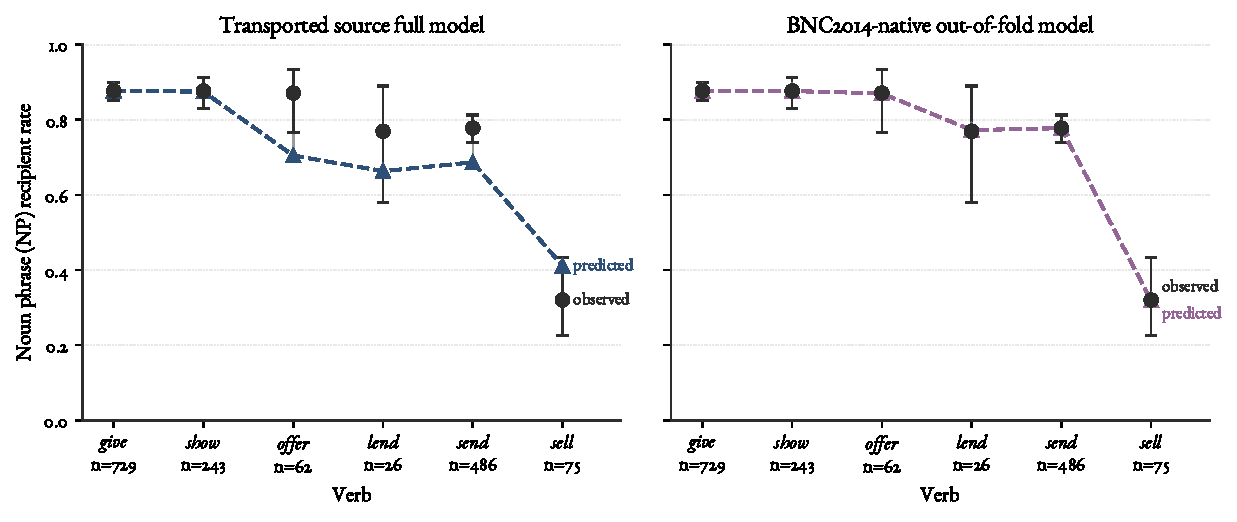
\includegraphics[width=\linewidth]{data/derived/figures/bnc2014_transport_calibration_by_verb.pdf}
\caption{Verb-level calibration for the transported \texttt{languageR} model
and the BNC2014-native holdout model. The vertical axis is the noun phrase
(NP) recipient rate. Sample sizes are shown under each verb.}
\label{fig:bnc-calibration}
\end{figure}

That framing changes the interpretation of the result. Success is evidence that
the conditioning profile is projectible across the bundled corpus shift within
the shared high-frequency core, not just refittable. Failure, if it had
occurred, would not have identified a single cause: variety, date, register,
verb restriction, and annotation all move together.

A scope limit bounds how far this generalizes. The six shared verbs are among
the most frequent and canonical members of the alternation, so transport is
tested where the conditioning profile is most likely to hold. The two datasets
intersect only on this high-frequency core; verbs with marginal, contested, or
idiosyncratic dative behaviour aren't shared, so they go untested here. The
result therefore licenses a claim about the core, not about the periphery, where
projectibility is hardest to establish.

The BNC2014-native model is still stronger. On a verb-stratified BNC2014
holdout split, the native core model reaches 0.202 log loss (bootstrap
[0.154, 0.254]) and 0.960 AUC (bootstrap [0.938, 0.979]). The gap is not small:
the transported model's log loss is about half again the native model's, and the
two bootstrap intervals don't overlap on either metric, so the difference isn't
just split noise. The transported model has learned a useful profile, but
BNC2014 also contains local structure that the \texttt{languageR} fit doesn't
capture.

Read the gap as a bounded downgrade rather than an apology. The transported
model clears the marginal and scrambled-label comparisons, so the result is not
just a same-corpus artefact. But the residual gap cannot be assigned to variety,
period, register, annotation, or the six-verb restriction one by one. Those
dimensions are bundled in this comparison.

Several directions travel. Recipient length is negative for NP realization;
theme length is positive; recipient pronominality is strongly positive; theme
pronominality is strongly negative; \texttt{sell} and \texttt{send} are less
NP-like than \texttt{give}. These are the strongest signs that the Bresnan
profile is projectible beyond one packaged dataset.

Some details do not travel cleanly. The transported model underpredicts NP
realization for \texttt{send}, \texttt{offer}, and \texttt{lend}, and
overpredicts it for \texttt{sell}. Theme definiteness is the clearest
coefficient mismatch: negative in the \texttt{languageR}-trained model, positive
and weak in the BNC2014-native model.

The recipient-definiteness proxy should stay a sensitivity check. Adding it
worsens transport log loss from 0.308 to 0.347 while leaving AUC essentially
unchanged. That pattern fits the harmonization note: the proxy is interpretable,
but it should not carry the headline result.

Acceptability evidence answers a different question. The Dative Alternation and
Information Structure (DAIS) dataset, introduced by
\textcite{HawkinsYamakoshiGriffithsGoldberg2020VerbBias}, contains 50,000 human
judgements over 5,000 dative sentence pairs and systematically varies verb,
definiteness, and argument length. The repository now carries a CC BY 4.0
licence, and the dataset authors have given explicit permission to reuse the
judgements. DAIS can therefore enter as a compact bridge
\citep{HawkinsYamakoshiGriffithsGoldberg2020DAIS}.

The bridge keeps the targets separate. I score only the 150 DAIS items whose
verbs overlap the six-verb production core. The same spoken \texttt{languageR}
production model that was transported to BNC2014 predicts a noun-phrase
recipient probability for each constructed DAIS pair; the DAIS item mean gives
the corresponding human double-object preference on a 0--1 scale. As a bridge
analysis, it asks whether a production probability profile and a controlled
preference profile point in the same direction.

\begin{figure}[htbp]
\centering
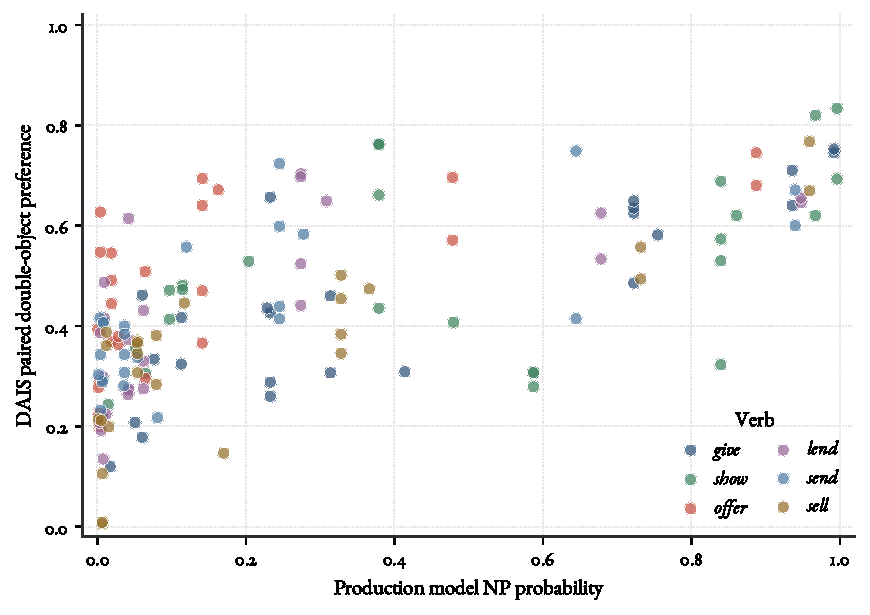
\includegraphics[width=0.82\linewidth]{data/derived/figures/dais_production_preference_bridge.pdf}
\caption{DAIS production/preference bridge for the six shared verbs. Each point
is a constructed DAIS item. The horizontal axis is the spoken
\texttt{languageR} model's noun phrase (NP) recipient probability; the vertical
axis is DAIS double-object (DO) preference. The diagonal marks equality between
the two channels, and the \mention{offer} cluster is highlighted because it
shows the clearest channel separation.}
\label{fig:dais-bridge}
\end{figure}

\begin{table}[htbp]
\centering
\small
\begin{tabular}{lrrr}
\toprule
Verb & Prod. NP prob. & DAIS DO pref. & Difference \\
\midrule
\mention{give} & 0.408 & 0.449 & -0.041 \\
\mention{lend} & 0.204 & 0.426 & -0.222 \\
\mention{offer} & 0.150 & 0.468 & -0.319 \\
\mention{sell} & 0.231 & 0.351 & -0.120 \\
\mention{send} & 0.196 & 0.428 & -0.232 \\
\mention{show} & 0.506 & 0.516 & -0.009 \\
\bottomrule
\end{tabular}
\caption{DAIS bridge for the six shared verbs. The DAIS column is the item-level
mean double-object (DO) preference. The production column is the noun-phrase
(NP) recipient probability from the spoken \texttt{languageR} core model.}
\label{tab:dais-bridge}
\end{table}

The two channels line up moderately, while remaining distinct. With
\mention{something} treated as a pronominal theme, Pearson's \(r\) is 0.667 and
Spearman's \(\rho\) is 0.685 over the 150 shared-verb items. The mean production
NP probability is 0.283, while the mean human DO preference is 0.440. Treating
\mention{something} as nonpronominal gives the same interpretation
(\(r = 0.645\), \(\rho = 0.675\), mean production probability 0.343).
The participant-level check points the same way without making the correlation
carry the whole inference. A mixed model on 1,525 shared-verb judgements from
923 participants, with random intercepts for participant and verb, is
non-singular; once recipient condition and theme type are included, the
incremental production-score coefficient is small (0.052, standard error
0.060). The bridge is therefore evidence of shared conditioning and diagnostic
divergence, not validation of one channel by the other.

The useful cases are the divergences. \mention{Offer} is the clearest verb-level
one: the production model makes it strongly PP-like, but DAIS participants are
much more willing to choose the double-object version. For example,
\enquote{Juan offered the woman a payment} has predicted NP probability 0.141
but DAIS DO preference 0.694. The point is channel separation: judgement
preference can occupy a different region of the evidence space from corpus
production probability.
